\section{Recurrent attention model} 

Our proposed model has four major components: A) a \textbf{2D external memory}
that tracks the state of the segmented objects; B) a \textbf{box proposal network}
responsible for localizing objects of interest;  C) a \textbf{segmentation network} 
for segmenting image pixels within the box; and D) a \textbf{scoring network} 
that determines if an object instance has been found, and also decides when to stop.
See Figure~\ref{fig:model_arch} for an illustration of these components.

\begin{figure}
\begin{center}
\begin{tabular}{cc}
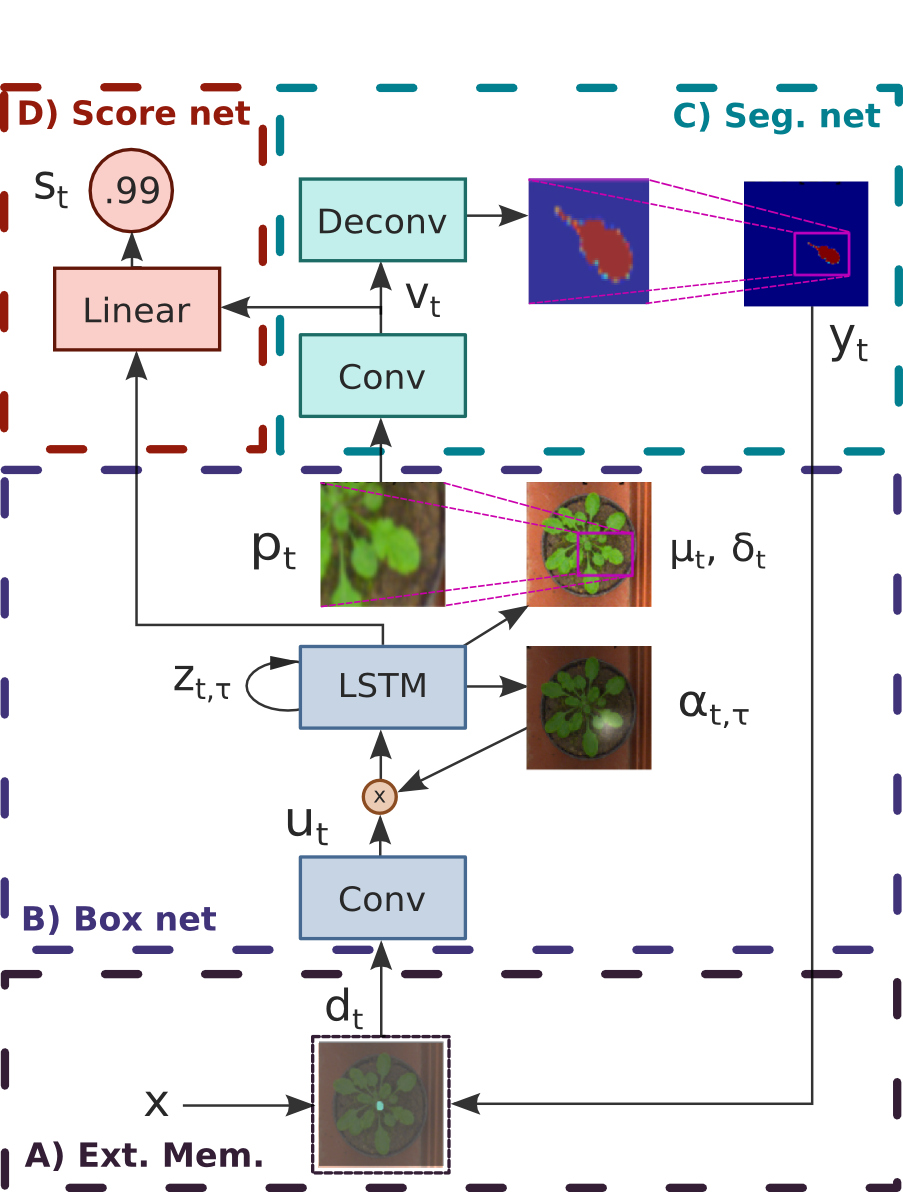
\includegraphics[width=0.52\textwidth]{./figs/model_arch.png} &
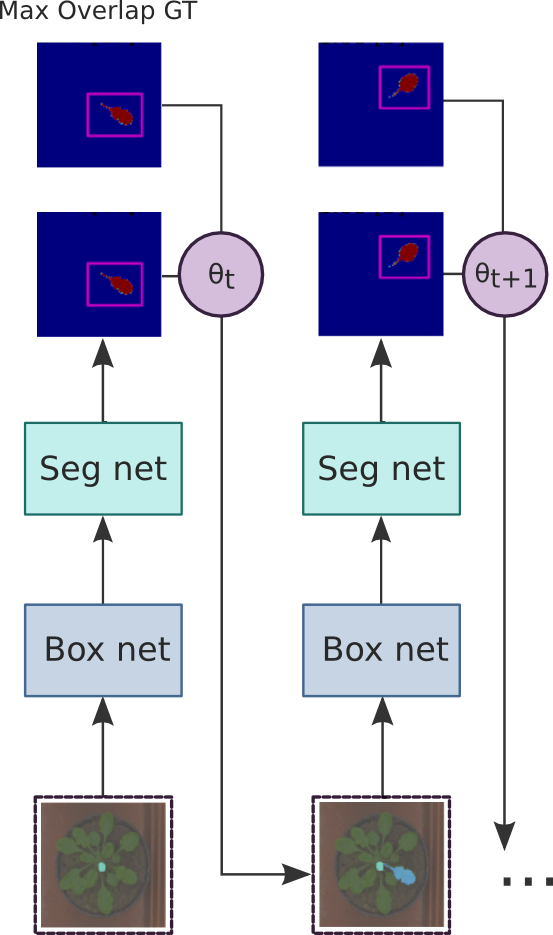
\includegraphics[width=0.38\textwidth]{./figs/model_arch2.png}
\end{tabular}
\end{center}
\caption{
Left: Detailed network design.
Right: Sketch of training, and scheduled sampling;
during training, the weighting of
ground-truth instance segmentations
relative to model predictions
($\theta_t$) decays to zero.
}
\label{fig:model_arch}
\end{figure}


\textbf{Notation}. We use the following notation to describe the model
architecture: $x \in \mathbb{R}^{H \times W}$
is the input image; $y_{t}$, $y^*_{t} \in (0, 1)^{H \times W}$ is the
segmentation  output/ground-truth sequence; $s_{t}$, $s^*_{t} \in (0, 1)$ is
the confidence score output/ground-truth sequence; $\mathcal{W}(z) = w^T z + b$ is a learned
affine transformation.

%%%%%%%%%%%%%%%%%%%%%%%%%%%%%%%%%%%%%%%%%%%%%%%%%%%%%%%%%%%%%%%%%%%%%%%%%%%%%%%
%%%%%%%%%%%%%%%%%%%%%%%%%%%%%%%%%%%%%%%%%%%%%%%%%%%%%%%%%%%%%%%%%%%%%%%%%%%%%%%
\subsection{Part A: Model input and external 2D memory}

We explore three variants of our model which differ in the first component. In
one formulation the input is the raw image, and in the others the image is fed
into a pretrained fully convolutional network (FCN). This \textbf{Pretrained
FCN} has two channels of output.  The first is a pixel-level foreground
segmentation, produced by a variant of the DeconvNet \cite{noh15deconv} with
skip connections. In addition to predicting this foreground mask, as a second
channel we followed the work of Uhrig et al. \cite{uhrig16insseg}  by producing
a 2-d object angle map. For each foreground pixel, we calculate its relative
angle towards the centroid of the object, and quantize the angle into 8
different classes, as shown in Figure~\ref{fig:fcn}. The angle map forces the
model to learn object boundary information, which is missing in the foreground
segmentation.  The architecture and training of these components are detailed
in the Appendix. We denote $D_0(x)$ as the pretrained FCN applied to the
original image.

\begin{figure}
\begin{center}
\resizebox{\columnwidth}{!}{
\begin{tabular}{ccc}

\includegraphics[width=0.5\textwidth]{./figs/fcn_out/fcn_input.png} &
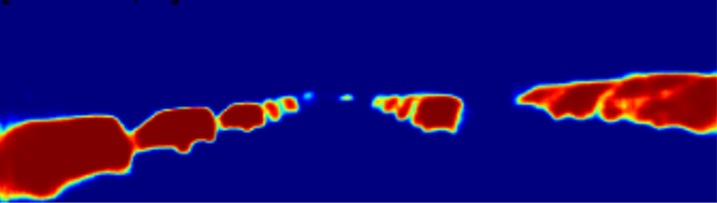
\includegraphics[width=0.5\textwidth]{./figs/fcn_out/fcn_seg.png} &
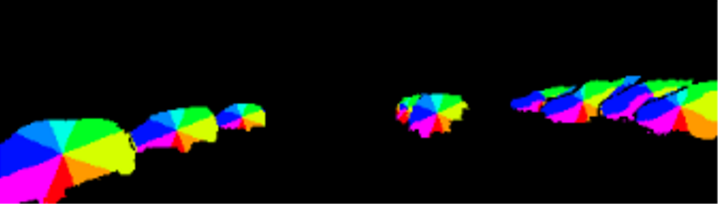
\includegraphics[width=0.5\textwidth]{./figs/fcn_out/fcn_angle.png}
\end{tabular}
}
\caption{Illustration of the output of the pretrained FCN. Left: input image.
Middle: predicted foreground. Right: predicted angle map.}
\label{fig:fcn}
\end{center}
\end{figure}


To facilitate learning to sequentially enumerate the objects, we incorporate an
external 2D memory in the RNN structure. We treat this 2D memory as the third
channel of the model input. We explore two alternative formulations of this
memory: 1) a \textbf{cumulative canvas} that stores the full history of
segmentation outputs, and 2) a \textbf{convolutional-RNN} with extra parameters
to dynamically adapt memory storage. Both operate at the full input resolution
to precisely deal with occlusion.

1. \textbf{\textit{Cumulative canvas}}. We hypothesize that providing
information of the completed segmentation helps the network reason about
occluded objects and determine the next region of interest. The first channel of
the canvas keeps adding new pixels from the output of the previous time step.
\vspace{-1pt}
\begin{align}
d_t^{\text{Canvas}} = \left[c_{t}, D_0(x)\right], \ \ \ \ 
c_0^{\text{Canvas}} &= 0, \ \ \ \
c_t^{\text{Canvas}} = \max(c_{t-1}, y_{t-1}) \ \forall t > 0
\end{align}
\vspace{-4pt}

2. \textbf{\textit{Convolutional LSTM}}. One issue of the cumulative canvas is
that the recurrent connection from the output of the previous time step into
the canvas sometimes leads to training instability. In practice, we observe
that reducing the gradient flowing back from the input of the canvas  aids
training. An alternative is to learn the ``addition'' operation with another
RNN. Convolutional LSTM \cite{shi2015convlstm} is a form of RNN that uses
convolution as its recurrent operator and thus is able to efficiently process
a 2D image input and store a 2D hidden state. We initialize the hidden state of
the ConvLSTM with the FCN output, and feed the output segmentation back
into the ConvLSTM (See Figure~\ref{fig:model_arch}, right). This allows the
gradient to flow through the ConvLSTM without introducing instability.
\vspace{-1pt}
\begin{align}
d_0^{\text{ConvLSTM}} &= D_0(x),\ \ \ \ 
d_{t}^{\text{ConvLSTM}} = \text{ConvLSTM}(d_{t-1}, y_{t-1}) \ \forall t > 0
\end{align}
\vspace{-6pt}

%%%%%%%%%%%%%%%%%%%%%%%%%%%%%%%%%%%%%%%%%%%%%%%%%%%%%%%%%%%%%%%%%%%%%%%%%%%%%%%
%%%%%%%%%%%%%%%%%%%%%%%%%%%%%%%%%%%%%%%%%%%%%%%%%%%%%%%%%%%%%%%%%%%%%%%%%%%%%%%
\subsection{Part B: Box network}

The box network localizes objects of interest. The CNN in the box network
outputs a $H' \times W' \times L$ feature map $u_{\text{box}, t}$. We employ a
``soft-attention'' mechanism here to extract useful information along spatial
dimensions and feed a dimension $L$ vector into the glimpse LSTM. Since one
single glimpse may not give the upper network enough information to decide
where exactly to draw the box, we allow the glimpse LSTM to look at different
locations.  $\alpha$ is  initialized to be uniform over all locations, and
$\tau$ indexes the glimpses.
\vspace{-1pt}
\begin{align}
u_{\text{box},t} = \text{CNN}(d_t), \ \ \ \
z_{t, \tau} &= \text{LSTM} (
\sum_{h, w} \alpha^{h, w}_{t, \tau} u^{h,w,l}_{\text{box},t}, z_{t, \tau-1} ), \ \ \ \
\alpha_{t, \tau+1} = \text{MLP}(z_{t, \tau})
\end{align}
\vspace{-6pt}

We pass the LSTM's hidden state through a linear layer to obtain predicted
box coordinates. We parameterize the box by its normalized center
$g_{X,Y}$, and log size $\log \delta_{X,Y}$. A scaling factor $\gamma$ is
also predicted by the linear layer, and used when re-projecting the patch
to the original image size.
\vspace{-1pt}
\begin{align}
(\tilde{g}_{X,Y}, \log \tilde{\delta}_{X,Y}, \log \sigma_{X,Y}, \gamma) &= \mathcal{W}(z_{t, \text{end}})
\end{align}
\begin{align}
g_X, g_Y &= (\tilde{g}_X+1)\frac{W}{2}, (\tilde{g}_Y+1)\frac{H}{2}, \ \ \ \  
\delta_X, \delta_Y = \tilde{\delta}_X W, \tilde{\delta}_Y H
\end{align}
\vspace{-6pt}

\textbf{Extracting a sub-region}. We follow DRAW \cite{gregor15draw} and use a
Gaussian interpolation kernel to extract a patch from the $\tilde{x}$, a
concatenation of the original image with $d_t$. We further allow the model to
output rectangular patches to account for different shapes of the object.
\begin{align}
\mu_X^i, \mu_Y^j &= g_X + (\delta_X + 1) \cdot (i - N / 2 + 0.5) / N, \ \  
g_Y + (\delta_Y + 1) \cdot (j - N / 2 + 0.5) / N
\end{align}
\begin{align}
F_X[a, i], F_Y[b, j] &= 
\frac{1}{\sqrt{2\pi} \sigma_X} \exp \left(- \frac{(a -
\mu_X^i)^2}{2\sigma_X^2} \right), 
\frac{1}{\sqrt{2\pi} \sigma_Y} \exp \left(- \frac{(b -
\mu_Y^j)^2}{2\sigma_Y^2} \right)
\end{align}
\begin{align}
p_t &= \text{Extract}(\tilde{x}_t, F_Y, F_X) \equiv F_Y^T \tilde{x}_t F_X
\end{align}
%\vspace{-6pt}

%%%%%%%%%%%%%%%%%%%%%%%%%%%%%%%%%%%%%%%%%%%%%%%%%%%%%%%%%%%%%%%%%%%%%%%%%%%%%%%
%%%%%%%%%%%%%%%%%%%%%%%%%%%%%%%%%%%%%%%%%%%%%%%%%%%%%%%%%%%%%%%%%%%%%%%%%%%%%%%
\subsection{Part C: Segmentation network}

The remaining task is to segment out the pixels that belong to the dominant
object within the window. In the segmentation network, we adopt a variant of
the DeconvNet \cite{noh15deconv} with skip connections, which appends
deconvolution (or convolution transpose) layers after convolution layers to
upsample the low-resolution feature map to a full-size segmentation. After the
fully convolutional layers, we get a patch-level segmentation prediction heat
map $\tilde{y}_t$. We then re-project this patch prediction to the original
image using the transpose of the previous computed Gaussian filters. The
learned $\gamma$ to magnifies the signal within the bounding box, and a
constant $\beta$ to suppresses the pixels outside the box. Lastly, the sigmoid
function produces final segmentation values between 0 and 1.
\begin{align}
y_t &= \text{sigmoid} \left(
\gamma \cdot \text{Extract}(\tilde{y}_t, F_Y^T, F_X^T)
- \beta \right)
\end{align}
%\vspace{-6pt}

%%%%%%%%%%%%%%%%%%%%%%%%%%%%%%%%%%%%%%%%%%%%%%%%%%%%%%%%%%%%%%%%%%%%%%%%%%%%%%%
%%%%%%%%%%%%%%%%%%%%%%%%%%%%%%%%%%%%%%%%%%%%%%%%%%%%%%%%%%%%%%%%%%%%%%%%%%%%%%%
\subsection{Part D: Scoring network}

To estimate the number of objects in the image, and to terminate our sequential
process, we incorporate a scoring network, similar to the one presented in
\cite{romeraparedes15ris}. Our scoring network takes information from the box
and segmentation network to produce a score between 0 and 1.
\begin{equation}
s_{t} = \text{sigmoid}(\mathcal{W}(z_{t, \text{end}}) + \mathcal{W}(u_{\text{segm}}))
\end{equation}
%\vspace{-4pt}

\textbf{Termination condition}. We train the entire model with a sequence length
determined by the maximum number of objects plus one. During inference, we cut
off iterations once the output score goes below 0.5. The loss function
(described below) encourages scores to decrease monotonically.
%\vspace{-4pt}

%%%%%%%%%%%%%%%%%%%%%%%%%%%%%%%%%%%%%%%%%%%%%%%%%%%%%%%%%%%%%%%%%%%%%%%%%%%%%%%
%%%%%%%%%%%%%%%%%%%%%%%%%%%%%%%%%%%%%%%%%%%%%%%%%%%%%%%%%%%%%%%%%%%%%%%%%%%%%%%
\subsection{Loss functions}

\textbf{Joint loss}. The total loss function is a sum of three losses:
the segmentation matching IoU loss $L_y$; the box IoU loss $L_b$;
and the score cross-entropy loss $L_s$:
\vspace{-3pt}
\begin{equation}
L(y, b, s) = L_y(y, y^*) + L_b(b, b^*) + L_s(s, s^*)
\end{equation}
\vspace{-4pt}

\textbf{(a) Matching IoU loss (mIOU)}. A primary challenge of instance segmentation
involves matching model and ground-truth instances.  we compute a
maximum-weighted 
bipartite graph matching between the output instances and ground-truth
instances \cite{stewart15lstmdet} and \cite{romeraparedes15ris}. Matching makes
the loss insensitive to the ordering of the ground-truth instances. Unlike
coverage scores proposed in \cite{silberman14insseg} it directly penalizes both
false positive and false negative segmentation. The matching weight $M_{i, j}$
is the IoU score between a pair of segmentation. We use the Hungarian algorithm
to compute the matching.
%\vspace{-3pt}
\begin{align}
M_{i, j} &= \text{softIOU}(y_i, y^*_j) \equiv \frac{\sum y_i \cdot y^*_j}
{\sum y_i + y^*_j - y_i \cdot y^*_j} \\
L_y(y, y^*) &= -\text{mIOU}(y, y^*) \equiv -\frac{1}{N} \sum_{i, j} 
M_{i, j} \mathbbm{1}[\text{match}(y_i) = y^*_j]
\end{align}
%\vspace{-12pt}

\textbf{(b) Soft box IoU loss}. Although the exact IoU can be derived from the 4-d
box coordinates, its gradient vanishes when two boxes do not overlap, which can
be problematic for gradient-based  learning. Instead, we propose a soft version
of the box IoU. We use the same Gaussian filter to re-project a constant patch
on the original image, pad the ground-truth boxes and compute the mIOU between
the predicted box and the matched padded ground-truth bounding box.
\vspace{-3pt}
\begin{align}
b_{t} &= \text{sigmoid}(\gamma \cdot \text{Extract}(\mathbf{1}, F_Y^T, F_X^T) -
\beta)\\
L_b(b, b^*) &= -\text{mIOU}(b, \text{Pad}(b^*))
\end{align}
%\vspace{-12pt}

\textbf{(c) Monotonic score loss}. To facilitate automatic termination, the
network should output more confident objects first. We proposed a loss function
that encourages monotonically decreasing values in the score output. Iterations
with target score 1 are compared to the lower bound of preceding scores, and 0
targets to the upper bound of subsequent scores.
\vspace{-3pt}
\begin{align}
L_s(s, s^*) &= \sum_t -s^*_t 
\log\left(\max_{t'=t...T-1} \{s_{t'}\}\right) - (1 - s^*_t)
\log\left(1 - \min_{t'=0...t} \{s_{t'}\}\right)
\end{align}
%\vspace{-12pt}

%%%%%%%%%%%%%%%%%%%%%%%%%%%%%%%%%%%%%%%%%%%%%%%%%%%%%%%%%%%%%%%%%%%%%%%%%%%%%%%
%%%%%%%%%%%%%%%%%%%%%%%%%%%%%%%%%%%%%%%%%%%%%%%%%%%%%%%%%%%%%%%%%%%%%%%%%%%%%%%
\subsection{Training procedure and post-processing}
\vspace{-3pt}

\textbf{Bootstrap training}. The box and segmentation networks rely on the
output of each other to make decisions for the next time-step. Because of the
coupled nature of the two networks, we propose a bootstrap training procedure:
these networks are pre-trained with ground-truth segmentation and boxes, 
respectively, and in later stages we replace the ground-truth with the model 
predicted values.

\textbf{Scheduled sampling}. To smooth out the transition between stages, we
explore the idea of ``scheduled sampling'' \cite{bengio15schedsamp} where we
gradually remove the reliance on ground-truth segmentation at the input of the
network. As shown in Figure~\ref{fig:model_arch}, during training there
is a dynamic switch in the input of the external memory, to utilize either the
maximally overlapping ground-truth instance segmentation, or the 
output of the network from the previous time step.

We denote $\theta_t$ as the probability of feeding in ground-truth segmentation
that has the greatest overlap with the previous prediction. $\theta_t$ follows
exponential decay as training goes on, and for larger $t$, the decays comes in
later.
\vspace{-3pt}
\begin{align}
\theta_t &= 
\min \left(\Gamma_t \exp \left(-\frac{step - S}{S_2} \right), 1 \right) \\
\Gamma_t &= 1 + \log(1 + Kt)
\end{align}

\textbf{Post-processing}. We truncate segmentation outside the predicted
foreground mask, fill holes with the labels from the nearest neighboring
predicted instance, and remove object segmentation of size smaller than 425
square pixels. We study the effect of post-processing in ablation studies in
Table~\ref{tab:kitti}.
